\documentclass[11pt, a4paper]{article}

 
\usepackage{amsmath, amssymb, amsthm, mathtools,pgfplots}
\usepackage{tikz}
\usepackage{pgfplots}
\usepackage{graphicx,caption,multicol}
\usepackage{verbatim}
%\usepackage{venndiagram}
\usepackage[cm]{fullpage}
\usepackage{color,enumerate,framed}
\usetikzlibrary{patterns}
\usepackage[labelfont=bf, labelsep=period]{caption}
%\captionsetup{labelformat=empty,labelsep=none}
\usepackage{mdwlist}
%\usepackage[nohug]{diagrams}
\usepackage[T1]{fontenc}
\usepackage{sidecap}
\usepackage[margin=1in]{geometry} 
%\usepackage{natbib}
\usepackage{hyperref}


\title{
	\vspace*{-1.5cm}
	\scshape 40.752 Algorithmic Game Theory\\
	\vspace{0.5cm}
	Project Proposal\\
	\vspace{0.5cm}
	{\bfseries\Large TO COOPERATE OR TO COMPETE: \\
		A GAME THEORETIC MODEL}\\
	\vspace{0.5cm}}

\author{Lai Zhangsheng \qquad \qquad Nguyen Tan Thai Hung}
\date{\today}

\begin{document}
	
	\maketitle
	\bibliographystyle{apalike}
	\section{Further development of Ideas}
	\subsection{Introduction}
	In a workplace, employers would ideally like their employees to cooperate and share knowledge with one another for various reason. Collaborative efforts between the employees promote better working relations and team bonding within the workplace. This helps to reduce the suspicion and tension between people with different job functions that arise from the lack of communication and understanding; a sectary that works in the usual working hours might mistake a fellow sales department colleague as slacking off when the sales colleague might be out doing sales most of the time and not in the office physically. Knowledge sharing between colleagues also allow one to be cross-trained in the duties of another, thus the company is able to function without much hiccups should an employee be away, since there are colleagues that are able cover for him or her. A cooperative effort amongst the employee is sometimes necessary as the whole is greater than the sum of its parts. With so much to be derived, it is understandable for the employers' push for cooperation.
	
	On the other hand, from the perspective of the employees, although they understand the employee's rationale for encouraging cooperation between them, the compensation scheme however, does not favour cooperation. Compensation schemes are typically based on the employee's key performance indicator (KPI) followed by a ranking based on it. An employee ranked higher would indicate a better monetary incentive and prospects of being promoted. It is tempting to associate a higher rank to a better job security, but such an association is not necessarily true. Companies are sometimes inclined to release a consistently highly ranked employee due to the huge cost of compensation and would instead prefer to use that resource to hire less experienced people as replacements. This sends the message to employees that being able to perform one's job function well might not necessarily be a good thing. The only way of maximising one's job security is to be irreplaceable and one way of being irreplaceable is to make one's role to be unique to ownself. This impedes the cooperation and knowledge sharing that is promoted by the employers but induces animosity and distrust between colleagues which thus lowers the social welfare of the company as a whole; the company performs less efficiently $-$ growth and profits of the company is thus impaired as a whole.
	
	From the observations made, we associate the strategy of cooperation and knowledge sharing as a optimal equilibrium and the strategy of being individualistic as a Nash equilibrium. Just like the scenario of a routing game, we see that the social cost is higher when the agents are only concerned about their cost as compared to when the agents are concerned about the social cost of the game. Hence in our model of the office game we would like to approach it in the flavour of a routing game and find some interesting bounds on the price of anarchy of such a game. We would also like to propose an appraisal mechanism that is incentive compatible which is the reason for the deviation towards the Nash equilibrium in the office games. In subsequent parts, `cooperation' will also mean knowledge sharing as knowledge sharing is also a form of cooperation.
	
	 
	
%	\begin{SCfigure}
%  \centering
%  \caption{ ... caption text ... }
% \begin{tikzpicture}
%		\begin{axis}[scale=1,
%		no markers,  domain=0:12, samples=100,
%		axis y line=center,
%		axis x line=center,
%		xlabel=$t$, ylabel=$p(t)$,
%		%every axis y label/.style={at=(current axis.above origin),anchor=south},
%		%every axis x label/.style={at=(current axis.right of origin),anchor=west},
%		%height=8cm, width=12cm,
%		%enlargelimits=true, 
%		clip=false,
%		axis equal,
%		xtick=\empty,
%		ytick=\empty,
%		ymin=-1,
%		% ymax=4,
%		xmin=0,
%		xmax=4,
%		%axis equal
%		%  minor tick num =5
%		]
%		%\addplot[mark=none,smooth,color=red,thick,domain=0:4] {1.7^x} 	node[pos=0.75,pin=150:{\color{black}$p(t)=a^t$},inner sep=0pt] {};
%		%\addplot[mark=none,smooth,color=blue,thick,domain=1:8] {ln(x)/ln(1.7)} node[pos=0.95,pin=-15:{\color{black}$p(t)=\log_a t$},inner sep=0pt] {};
%		\addplot[thick,dashed,domain=0:3] {x} node[pos=0.95,pin=45:{\color{black}$p(t)=t$},inner sep=0pt] {};
%		\end{axis}
%		\end{tikzpicture}
%		\end{SCfigure}
%	the employer would ideally like the employees to cooperate with one another as the expected efficiency gains is 
	\subsection{The model}
	The approach to formulating our model would be to first identify the properties that we like to have in the compensation schemes that will favour deviation to a more cooperative environment after which we will construct the model that fits our desired requirements. To simply the complexity of this problem, we shall consider the scenario where there are two agents (employees) 1 and 2. We do not like \cite{Chakravarti2015}, consider the role of an employer, which maximises the utility of the employer at the expense of the utility of the agents. Our focus is on how investigating how bad the game is in price of anarchy terms and how a better design of this game can improve the price of anarchy.
	
	
	
	
	\cite{Chakravarti2015}
	\cite{Drago1991}
	
	\section{Motivation}
	The idea for this project is drawn upon our own observation from past work experiences. In the workplace, managers typically want their staff to cooperate with one another in order to achieve a good overall performance for the company. However, staff appraisals are often done according to a bell curve, which disincentifies people to cooperate: if a worker helps his colleague, he faces stronger competition for the top ranks. This appraisal mechanism is thus not incentive compatible. A similar phenomenon is observed in the classroom context. Students should study together and help each other, but the bell curve system can cause competition among students, leading to poorer learning outcomes. In this project, we want to model what happens in the workplace from a game theoretic perspective. Then, we will attempt to figure out a way to quantify the performance, and propose a better mechanism. 
	
	Certainly, there are situations in which competition increases production, such as what was observed in the steel factory of Charles M. Schwab\footnote{Netessine and Yakubovich. The Darwinian workplace. \textit{Harvard Business Review}. \url{https://hbr.org/2012/05/the-darwinian-workplace}}. For each shift, Schwab wrote on the factory floor the amount of steel the previous shift had produced. The night shift workers, upon seeing the number from the day shift, worked themselves hard so as to break the record set by the day shift. Soon, the two shifts were trying their best to out perform each other for bragging rights, and production soared. Schwab's method may have worked back in those days, but may not be applicable in a modern day's context. In fact, as Dan Pink\footnote{Dan Pink. The puzzle of motivation (TED Talk). \url{https://youtu.be/rrkrvAUbU9Y}} pointed out, incentives may boost productivity if the task only requires linear thinking and individual focus. However, the workplace environment nowadays increasingly requires nonlinear thinking and collaborative efforts. This work considers a modern workplace setting where everyone receives, a part from their fixed remuneration, a variable reward (e.g. financial bonus or job promotion) that depends on his own performance relative to those of his colleagues, as well as the performance of the company as a whole. Everyone wants to rise up the ranks, and the strategy employed by the general population seems to move towards individualistic competition so as to outshine their colleagues.
	
	\section{Model}\label{sec:model}
	\subsection{A general model}
	We shall consider a workplace reward maximizing game where there are $k$ agents, each of whom is assigned a specific project. Every agent $i$ is assumed to have the same time budget $T$, and he dedicate some of his time to his own project and some to his colleagues'. As a result, he has a time distribution (from here on referred to as a \textit{schedule)}, which is a vector $t_i=(t_{i1},t_{i2},\ldots,t_{ik})$  where $t_{ii}$ denotes the time agent $i$ allocates to his own project and $t_{ij}$ represents the time allocated by agent $i$ to agent $j$'s project, and $\sum_{j=1}^{k}t_{ij}=T$.	
	
	For each project $j$, its work output (performance) is a function of the total time effort dedicated to it. To reflect the diminishing returns of time investment, we use the natural logarithm to express this relationship (Figure \ref{fig:log}).
	\begin{equation}\label{eq:pj}
		p_j = \beta_j\log\left(t_{jj}+\sum_{i\neq j}^{k}\alpha_{ij}t_{ij}\right)
	\end{equation}
	where $\alpha_{ij}$ is the effectiveness (as a result of skill or experience) of agent $i$ when working on project $j$, compared to that of the project owner, and $\beta_{j}$ is a coefficient that reflects the value of the project. Agents are ranked according to his own project's performance. A higher rank means a higher reward. In addition, the reward is also affected by the company's performance as a whole.	
	\begin{equation}\label{eq:ui}
		u_i=f(r_i, P)
	\end{equation}
	where 
	\begin{itemize}
		\item $r_i$ is the rank of agent $i$ compared to his colleagues. $r_i$ can be obtained by cardinal ranking, by means of a bell curve, or byt any other ranking methods, and
		\item $P$ is the company performance, which, for simplicity, is taken as the total performance of all its employees, $P=\sum_{i}p_i$. 
	\end{itemize}
	\begin{figure}
		\centering
		\begin{tikzpicture}
		\begin{axis}[scale=0.75,
		no markers,  domain=-1:12, samples=100,
		axis y line=center,
		axis x line=center,
		xlabel=$t$, ylabel=$p(t)$,
		every axis y label/.style={at=(current axis.above origin),anchor=south},
		every axis x label/.style={at=(current axis.right of origin),anchor=west},
		height=8cm, width=12cm,
		enlargelimits=true, 
		clip=false,
		axis equal,
		xtick=\empty,
		ytick=\empty,
		ymin=-1,
		% ymax=4,
		xmin=-1,
		xmax=4,
		%axis equal
		%  minor tick num =5
		]
		\addplot[mark=none,smooth,color=red,thick,domain=0:4] {1.7^x} 	node[pos=0.75,pin=150:{\color{black}$p(t)=a^t$},inner sep=0pt] {};
		\addplot[mark=none,smooth,color=blue,thick,domain=1:8] {ln(x)/ln(1.7)} node[pos=0.95,pin=-15:{\color{black}$p(t)=\log_a t$},inner sep=0pt] {};
		\addplot[thick,dashed,domain=0:8] {x} node[pos=0.95,pin=45:{\color{black}$p(t)=t$},inner sep=0pt] {};
		\end{axis}
		\end{tikzpicture}
		\caption{Comparison between diminishing return (blue), linear return (black) and exponential return (red).}\label{fig:log}
	\end{figure}

	\subsection{Routing game equivalent}
	We will prove that this game is equivalent to an atomic routing game. The time budget could be though of as the commodity of an agent and the agent needs to route all its commodity through a single source and sink network with parallel links. Each edge linking the source and sink represents a project and when an agent chooses to route some `flow' through a particular edge, it is just same as saying that the agent is investing time into that project (Figure \ref{fig:network}). This equivalence guarantees that a pure Nash equilibrium exists.
	\begin{figure}[h]
		\centering		
		\def\layersep{2.5cm}		
		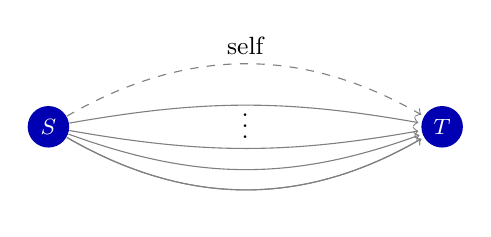
\begin{tikzpicture}[scale = 1,shorten >=1pt,->,draw=black!50, node distance=\layersep]
		\tikzstyle{every pin edge}=[<-,shorten <=1pt]
		\tikzstyle{neuron}=[circle,fill=black!25,minimum size=15pt,inner sep=0pt]
		\tikzstyle{output neuron}=[neuron, fill=red!50];
		\tikzstyle{n}=[neuron, fill=blue!70!black];
		
		\node[n] (a) at (0,0) {\color{white}{\footnotesize $S$}};
		\node[n] (b) at (5,0) {\color{white}{\footnotesize $T$}};
		\draw (a) edge[bend left, dashed] node[above] {\small self } (b);
		\draw (a) edge[bend right=-10] node[above] {\small } (b);
		
		\draw (a) edge[bend right=10] node[above] {\small $\vdots$} (b);
		\draw (a) edge[bend left=-20] node[above] {\small } (b);
		\draw (a) edge[bend left=-30] node[above] {\small } (b);
		\draw (a) edge[bend right] node[below] {\small } (b);
		\end{tikzpicture}
		\caption{An equivalent routing game}\label{fig:network}
	\end{figure}

	\subsection{A toy example}
	We will investigate the simplest instantiation of the model: a two-agent case, for which different scenarios concerning $\beta_i$ and $\alpha_{ij}$ will be investigated. The optimal and equilibrium strategies will be determined and the Price of Anarchy as well as its bound will be analysed.
	
	In a two-agent case, it is important to distinguish our model from the well-known Prisoners' Dilemma
	
   %	The Prisoners' Dilemma's payoff table is 
	%	\begin{table}[h]
	%		\centering
	%		\caption{Prisoners' Dilemma's payoff table}
	%		\begin{tabular}{c c c}
	%			& Silent & Betray \\
	%			Silent  & 1, 1    & 3, 0     \\
	%			Betray  & 0, 3    & 2, 2
	%		\end{tabular}
	%	\end{table}
	%	
	%	The payoff table of our game is still to be determined, but we believe that there are some differences, and we may want to tackle some or all of them
	\begin{itemize}
		\item In the Prisoners' Dilemma game, players can move only once and they are not allowed to talk to each other. In our game, both these constraints are not present.
		\item The Prisoners' Dilemma is symmetric, while it is reasonable to assume that our two office workers are different in many ways. For example, they have different skill sets.		
	\end{itemize}
	
	%\emph{Here, we would like to address some of the assumptions that have been made which might have to lead to some scenarios of a real office setting not being considered in this model. }	
	\section{Mechanism design}
	After determining the performance of the existing reward scheme, we will attempt to propose a different reward scheme such that cooperation becomes the dominant strategy. We draw our inspiration from real life games such as World of Warcraft and DOTA, where we have seen cooperative efforts to achieve the game objectives. Hence, we hope to transfer what was applied in the games to the workplace setting.
	
	\subsection{Fitting into an atomic routing game scenario}
	The properties of an atomic routing game is well known to us and by trying to fit the model of our problem into the structure of a routing game, we hope to gain better insight and better understanding of the model of the office games we proposed in Section \ref{sec:model}.
	
	\newdimen\R
\R=2cm
\begin{figure}[h]
	\centering
	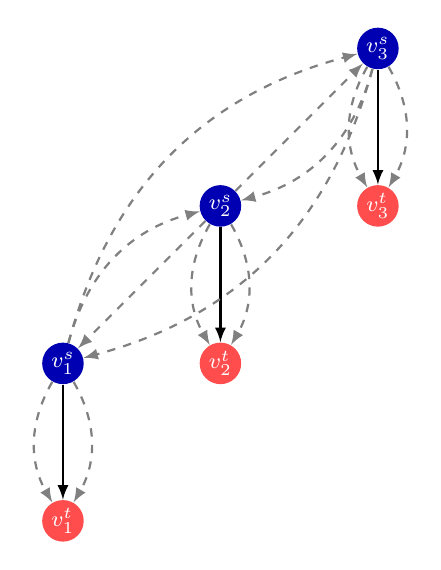
\begin{tikzpicture}[scale=1,draw=black!50,>=latex]
	\tikzstyle{neuron}=[circle,fill=black!25,minimum size=15pt,inner sep=0pt]
	\tikzstyle{m}=[neuron, fill=blue!70!black];
	\tikzstyle{n}=[neuron, fill=red!70!white];
%	\foreach \x in {1,2,3}{
%	\node[m,yshift=\x*2 cm](s-\x) at (\x*2-2*2,1){\footnotesize {\color{white}$s_{\x}$}};
%	\node[n,yshift=\x*2 cm](t-\x) at (\x*2-2*2,-1){\footnotesize {\color{white}$t_{\x}$}};
%	}
%	
	\node[m,yshift=2 cm](s-1) at (-2,1){\footnotesize {\color{white}$v^s_1$}};;
	\node[m,yshift=4 cm](s-2) at (0,1){\footnotesize {\color{white}$v^s_2$}};
	\node[m,yshift=6 cm](s-3) at (2,1){\footnotesize {\color{white}$v^s_3$}};
	\node[n,yshift=2 cm](t-1) at (-2,-1){\footnotesize {\color{white}$v^t_1$}};
	\node[n,yshift=4 cm](t-2) at (0,-1){\footnotesize {\color{white}$v^t_2$}};
	\node[n,yshift=6 cm](t-3) at (2,-1){\footnotesize {\color{white}$v^t_3$}};
	\foreach \x in {1,2,3}{
	\draw[->,color=black,thick] (s-\x) -- (t-\x);
	\draw[->,thick,dashed] (s-\x) edge[bend right] (t-\x);
	\draw[->,thick,dashed] (s-\x) edge[bend left] (t-\x);
	}
	\draw[->,thick,dashed] (s-1) edge[bend left] (s-2);
	\draw[->,thick,dashed] (s-1) edge[bend left] (s-3);
	\draw[->,thick,dashed] (s-2) edge (s-3);
	\draw[->,thick,dashed] (s-2) edge (s-1);
	\draw[->,thick,dashed] (s-3) edge[bend left] (s-2);
	\draw[->,thick,dashed] (s-3) edge[bend left] (s-1);
	\end{tikzpicture}
	\caption{Office game seen as a routing game with 3 agents}
	\label{fig:officerouting}
\end{figure}

%\begin{figure}[h]
%	\centering
%	\begin{tikzpicture}[scale=1.5,draw=black!50]
%	\tikzstyle{neuron}=[circle,fill=black!25,minimum size=15pt,inner sep=0pt]
%	\tikzstyle{m}=[neuron, fill=blue!70!black];
%	\tikzstyle{n}=[neuron, fill=red!70!white];
%	\foreach \x in {1,2,3}{
%	\node[m,yshift=\x*2 cm](s-\x) at (\x*2-2*2,1){\footnotesize {\color{white}$s_{\x}$}};
%	\node[n,yshift=\x*2 cm](t-\x) at (\x*2-2*2,-1){\footnotesize {\color{white}$t_{\x}$}};
%	}
%	\foreach \x in {1,2,3}{
%	\draw[->] (s-\x) -- (t-\x);
%%	\draw[->] (s-\x) edge[bend right] (t-\x);
%%	\draw[->] (s-\x) edge[bend left] (t-\x);
%	}
%%	\draw[->] (s-1) edge[bend left] (s-2);
%%	\draw[->] (s-1) edge[bend left] (s-3);
%%	\draw[->] (s-2) edge (s-3);
%%	\draw[->] (s-2) edge (s-1);
%%	\draw[->] (s-3) edge[bend left] (s-2);
%%	\draw[->] (s-3) edge[bend left] (s-1);
%	\end{tikzpicture}
%	\caption{Office game seen as a routing game}
%	\label{fig:bipartite}
%\end{figure}


	In such a routing game, we have $G=(V,E)$, where $V$ and $E$ are the usual set of vertices and edges respectively. A usual routing game will require a player to route his commodity from $s_i$ to $t_i$; ours is similar but with some constrains:
	\begin{itemize}
	\item an agent $j$ is only allowed to route from a single source that is unique to him, this vertex $v^s_j$ represents the agent himself or herself.
	\item any edge from $v^s_j$ can only be directed to:
	\begin{itemize}
	\item	 the unique vertex $v^t_j$ which represents the agent's assigned project, or
	\item a vertex $v^s_k$, that represents another agent, which then there must be another edge from $v^s_k$ to $v^t_k$. This represents cooperation between $v^s_j$ and $v^s_k$ (agents $k$ and $j$), with the first edge of the path $v^s_j\to v^s_k$ represent some form of cooperation utility and the second $v^s_k\to v^t_k$ representing the contribution of agent $j$'s time to agent's $k$ project.
	\end{itemize}
	\end{itemize}
	The solid directed edges in Figure \ref{fig:officerouting} denotes an agent's investment of time into the agent's own project. The dotted lines represents the edges formed when cooperation occurs. With this idea, we want to see the correspondence between our office games and routing games to gain a better understanding of how bad office games can get.
	\section{Experiment} 
	This may be somewhat too ambitious, but we hope to conduct an experimental game on the \href{http://arenalabs.co/}{ArenaLabs} website to verify our model.
	
	\section{Theoretical background}
	The problem was first mentioned in literature by \cite{Drago1991}. Since this seminal work, several scholars have investigated the problems in deeper details:
	\begin{itemize}
		\item \cite{Drago1998} and \cite{Kistruck2016} discuss different reward structures to encourage cooperation.
		\item \cite{Banerjee2014} and \cite{Chakravarti2015} also explore incentive schemes, but with focus on knowledge sharing among researchers and team members.
		\item \cite{Immorlica2011} discussed a dueling game and show how bad head-on competition can get.
		\item \cite{Landers2015} described an interesting gamification experiment to understand how people actually behave when the reward mechanism is changed.		
	\end{itemize}
	\newpage
	\bibliography{AGT_project}
	\bibliographystyle{apalike}

\end{document}
